\documentclass[a0paper,portrait]{tikzposter}
\usepackage[T1]{fontenc}
\usepackage[utf8]{inputenc}
\usepackage[french]{babel}
\usepackage[backend=bibtex,doi=false,isbn=false,url=false]{biblatex}
\addbibresource{../montecarlo-simulation.bib}
\usepackage{graphicx}

\usepackage{acronym}
\acrodef{mcs}[MCS]{Monte-Carlo simulation}
\acrodef{btu}[BTU]{billing time unit}

\title{\parbox{\linewidth}{\centering{}
	An overview of Cloud Simulation Enhancement using the Monte-Carlo Method
	}
}
\institute{\texttt{\{lbertot,genaud,gossa\}@unistra.fr}\\
	ICube laboratory \textendash{} University of Strasbourg, CNRS
	} % See Section 4.1
\author{Luke Bertot, Stéphane Genaud, Julien Gossa}   
%\titlegraphic{Logo}
%\usetheme{default}  % See Section 5
\colorlet{backgroundcolor}{white}
%\usetitlestyle{Wave}
\begin{document}
\maketitle  % See Section 4.1
\begin{columns}
  \column{0.65} \block{1. Running Scientific Workflows in the Cloud}{%See Section 4.2
	 The Cloud gives access to instantaneous on-demand computing power, with
	 a rental cost directly proportional to resource's use-time, counted
	 in \ac{btu}. Like all shared-tenancy platforms, IaaS platforms
	 present a significant variability~\cite{LeitnerC16}.\\

	 We developed Schlouder~\cite{Michon17}, a cloud broking system capable
	 of scheduling batch-jobs to IaaS clouds. Schlouder schedules tasks,
	 provisions resources, and monitors the tasks and the VMs life cycles.
	 The scheduling and provisioning is controlled by an heuristic called
	 \emph{Strategy}, which can be used to favor shorter makespans (total 
	 runtime) as in ASAP, or lower cost (less BTU) as in AFAP.\\  

	 Strategies are not uniformly efficient and some heuristic fail to
	 perform well with certain workflows. Because of the 
	 \emph{pay-as-you-go} model of IaaS clouds, the simulation of job is 
	 critical tool to select the appropriate strategy. However the 
	 variability of cloud platforms is not taken into account by the 
	 discrete event simulations usually used.\\

	 On a private 96-core Openstack cloud, we ran 200 instances of 
	 OMSSA~\cite{Geer2004}, used for the analysis of mass-spectrometer 
	 results, using alternatively the ASAP and AFAP strategies. 
	Figure 1.\ presents the distributions of makespan (in seconds) and cost 
	(in number of BTU) observed during these runs. 
}
\column{0.35}
\block{}{%
	\begin{tikzfigure}[Makespan and cost distribution for real runs of 
		OMSSA.]
		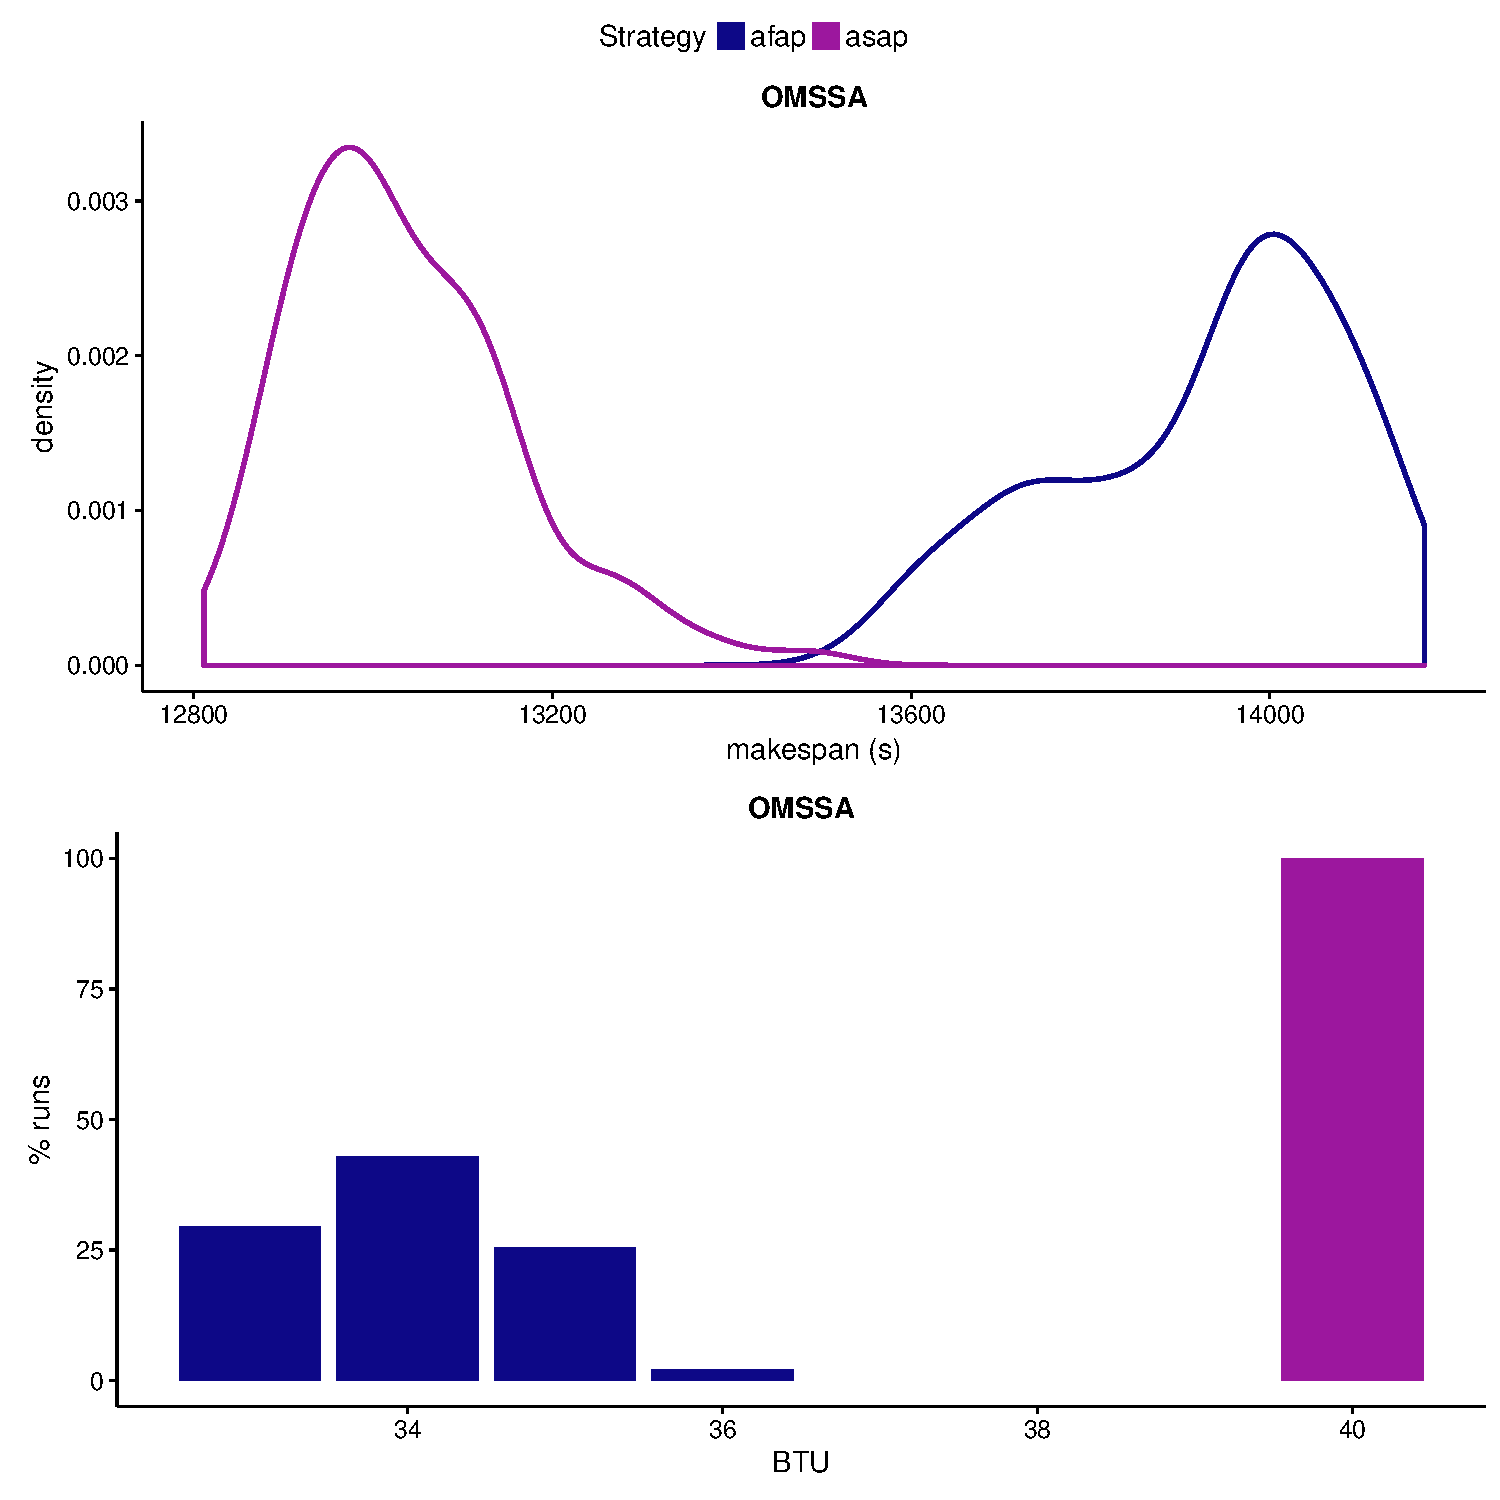
\includegraphics[width=0.87\linewidth]{gfx/PP_real.pdf}
	\end{tikzfigure}
}
\end{columns}


\begin{columns}  % See Section 4.4

\column{0.6}  % See Section 4.4

\block{2. Monte-Carlo Simulation}{%
	Using Simgrid~\cite{simgrid} we developed a IaaS cloud simulation 
	framework, SchIaaS. We used SchIaaS to create SimSchlouder, a simulation
	of Schlouder. SimSchlouder reproduces the scheduling, provisioning, and
	strategies of Schlouder. But as a discrete event simulator SimSchlouder
	does not account for the inherent variability of task runtimes. 

	In stochastic simulations the task runtimes are replaced by runtime
	distributions, representing all possible runtimes and their relative
	likelihood. A numerical solution to these simulations is exists in cases
	where the distribution of every task is independent and scheduling is
	static.

	\ac{mcs} can be used to perform stochastic simulations, without the
	constraints of the numerical solutions and using a deterministic 
	simulator. A \ac{mcs} work by sampling possible simulation results, by
	simulating \emph{realizations}. A realization is a possible scenario of
	a job execution, and is obtained by drawing a value from each input 
	distribution. The simulation of a realization is entirely deterministic
	and can be done using any classic cloud simulator.

	In this case our input distributions are the tasks runtimes.\\
\begin{tikzfigure}[A 500 iteration Monte-Carlo simulation.]
	\begin{tikzpicture}[
sim/.style={%
draw, 
rounded corners
}
]
%% Origin node
\node[align=center]at(0,2){Job\\RVs};
\node at(0,0)(orig){$\{R_1,\ldots,R_n\}$};
%% Realisations
\node at(3.5,2){Realisations};
\node[]at(3.5,1)(pert1){$\{T_1^1,\ldots,T_n^1\}$};
\node at(3.5,0){\vdots};
\node at(3.5,-1)(pert5){$\{T_1^{500},\ldots,T_n^{500}\}$};
\draw[-{latex}](orig)--(pert1);
\draw[-{latex}](orig)--(pert5);
%%
\node[sim]at(6,1)(s1){Sim};
\node[sim]at(6,-1)(s5){Sim};
\node at(6,0){\vdots};
\draw[-{latex}](pert1)--(s1);
\draw[-{latex}](pert5)--(s5);
%% Makespans
\node at(8,2){Samples};
\node at(8,1)(M1){$M^1$};
\node at(8,-1)(M5){$M^{500}$};
\node at(8,-0){\vdots};
\draw[-{latex}](s1)--(M1);
\draw[-{latex}](s5)--(M5);
%% Consolidation
\node[align=center]at(10,2){Makespan\\RV};
\node at(10,0)(r){$M_S$};
\draw[-{latex}](M1)--(r);
\draw[-{latex}](M5)--(r);
%%phases
\node[align=center]at(1.75,-2.5)(df){realisation\\draw};
\draw[dotted](1.75,1.5)--(1.75,-2);
\node[align=center]at(9,-2.5)(df){distribution\\fitting};
\draw[dotted](9,1.5)--(9,-2);
\end{tikzpicture}

\end{tikzfigure}
}
\block{4. Results}{%
	Figure 3.\ presents the distribution of makespans and costs obtained
	with 500 \ac{mcs} iterations using our task model, and compares them to
	the distributions observed in real executions.

	We can quantify our capture rate on the makespan using statistical 
	fitting. By fitting our \ac{mcs} result to a Normal distribution we 
	produce confidence intervals (CI). The 95\%CI captures 90\% of real 
	execution in ASAP and 92\% in AFAP. Using the 99\% CI yields capture 
	rates of 98\% and 100\%	respectively.

	The discrepancy between the nominal capture rate of the interval and the
	proportion of real execution captured can be partly explained by fitting
	error as the distribution of real execution makespans slightly differs
	from a Normal distribution. The simple task model is also a limiting factor. 
	Figure 3.\ shows that even when the capture rate is 100\% as is the case
	with BTU cost, the distribution is not the same. This is the results of
	simplification caused by the task model.  
}
\block{5. In Short}{%
	IaaS Clouds present inherent variability which affects the cost and time
	necessary to run a job. This variability is a serious impediment to the
	use of simulators as prediction tools.\\

	Using a simple task model Monte-Carlo simulations allows us to account 
	for the variability of a job executed on the cloud with sufficient 
	precision to capture 90\% of real runs.
}
\column{0.4}
\block{3. Task Model}{%
	We chose to model our tasks using simple uniform distributions. Each
	distribution is centered on the average expected runtime for that task
	($\bar{r}_t$). The relative spread of each distribution represents the
	expected platform variability and is called the perturbation level ($P$).
	As such the distribution $R_t$ for a task $t$ is expressed as :	
	\[R_t = \mathcal{U}(\bar{r_t}\cdot{}(1-P),\bar{r_t}\cdot{}(1+P))\]
	We computed the expected variability of our platform as being the 
	average across all tasks of the worst-case deviation from 
	the expected value for each task. On our platform $P\approx10\%$.

	We show that this simple model is sufficient to obtain accurate simulation
	results. 
} 
\block{}{%
	\begin{tikzfigure}[Distribution of makespans and costs computed by the \ac{mcs}]
	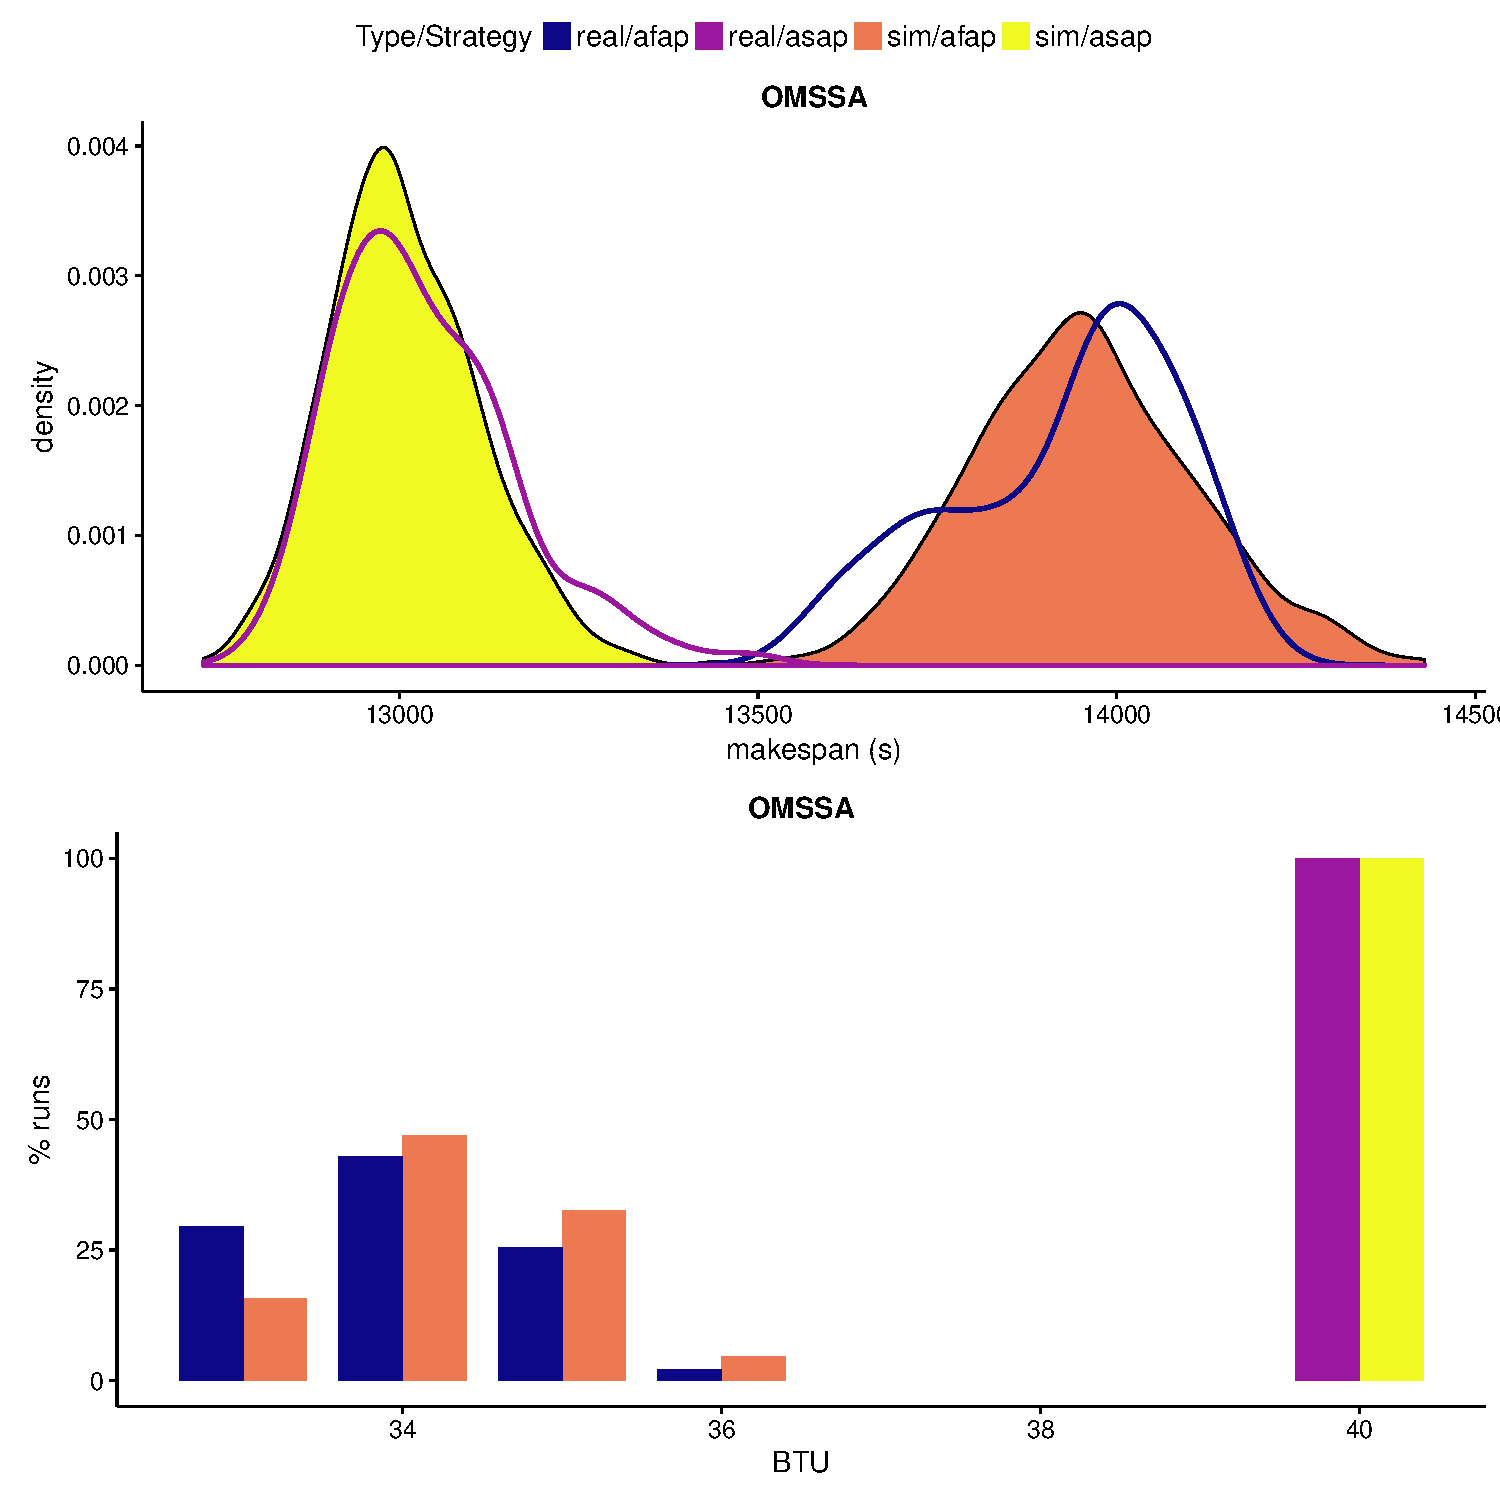
\includegraphics[width=0.9\linewidth]{gfx/PP_fit.pdf}
\end{tikzfigure}
}
\block{References}{\printbibliography[heading=none]}
\end{columns}

\end{document}
% vim:spell spelllang=en:
